\documentclass[12pt]{article}
\usepackage{amssymb,graphicx}
\usepackage{subfigure}
\usepackage[hyphens,obeyspaces,spaces]{url}
\usepackage{amsmath}
\usepackage{amsfonts}
\usepackage{amssymb}
\usepackage[T1]{fontenc}
\usepackage{carolmin}
\usepackage{t1enc}
\usepackage{color}
%\usepackagqe{times}
\usepackage{textcomp}
%\usepackage{natbib}

\def\eop{\hfill{$\vcenter{\hrule height1pt \hbox{\vrule width1pt
height5pt \kern5pt \vrule width1pt} \hrule height1pt}$}}

\newcommand{\bydef}{\mbox{$\:\stackrel{\triangle}{=}\:$}}
\newcommand{\insmat}[1]{\mathop{\rm {#1}}}  % for mathmode (with underlines)
\newcommand{\half}{{\textstyle\frac{1}{2}}}
\newcommand{\norm}[1]{\|#1\|}
\newcommand{\argmin}{\insmat{arg\,min}}
\newcommand{\argmax}{\insmat{arg\,max}}
\newcommand{\dist}{\insmat{dist\,}}
\newcommand{\aff}{\insmat{aff\,}}
\newcommand{\cl}{\insmat{cl\,}}
\newcommand{\conv}{\insmat{conv\,}}
\newcommand{\Qh}{\widehat{{\Omega}}}
\newcommand{\gammapQ}{\gamma_{p {\Omega}}}
\newcommand{\Pmu}{\mathbb{P}_\mu}
%\linespread{3.0} %For JOTA format


\begin{document}
%\noindent
%\begin{center}
%\large \textbf{Suboptimality of minmax MPC}
%\vspace{0.5cm}
%\noindent
%\vspace{0.5cm}
%\end{center}

\noindent
\begin{center}
 \textbf{Obstacle Avoidance Constraint in Lateral Controller}
\vspace{0.5cm}
\noindent
\vspace{0.5cm}
\end{center}
%CHAGE $\bold{u_{t}}$ to something like $u^{t}$ or $u_{t}$
I think following function can be easily incorporated to the current lateral MPC controller in order to provide collision avoidance capability. 
Let $x(t)$ and $\tau$ be a vehicle position at time $t$ and a obstacle position, respectively. Two variables $\alpha$ and $s$ are tuning parameters. The scalar value $w$ is a weight parameter.

\begin{equation}
z(t) = w\frac{\exp(-\alpha(\|x(t)-\tau\|^2-s^2))}{1+\exp(-\alpha(\|x(t)-\tau\|^2-s^2))}
\end{equation}

$z(t)$ applies large penalty to the position of the obstacle that is located at $\tau$. Therefore, this term can be added in the cost function. Alternatively, we can use this term as a hard constraint, $i.e.$ $z(t) \leq \bar{z}$, where $\bar{z}$ is minimum allowed distance to the obstacle.

Fig.1 and Fig.2 shows the effect of two tuning parameters $s$ and $\alpha$.
horizontal axis is $x$, vertical axis is $z$ for both Fig.1 and 2.
\begin{figure}[h!]
\begin{centering}
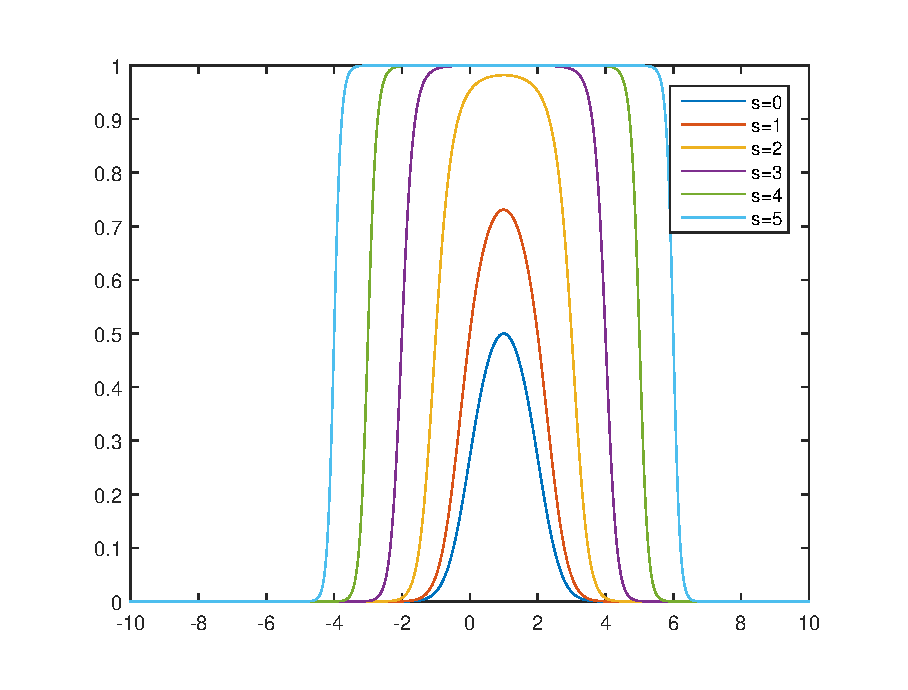
\includegraphics[width=12cm]{./Figures/bell1.eps}
\par\end{centering}
\caption{Obstacle penalty term parametrized by $s$.}
\end{figure}
As shown in Fig.1 the parameter $s$ determines the range of penalty effect.

\begin{figure}[h!]
\begin{centering}
\includegraphics[width=12cm]{./Figures/bell2.eps}
\par\end{centering}
\caption{Obstacle penalty term parametrized by $\alpha$.}
\end{figure}
As shown in Fig.2 the parameter $\alpha$ determines growing rate of the penalty.

\end{document}